
\documentclass[journal,comsoc]{IEEEtran}
\usepackage[T1]{fontenc}
\usepackage{url}
\usepackage{graphicx}
\usepackage{float}
\ifCLASSINFOpdf
\else
\fi
\usepackage{amsmath}
\interdisplaylinepenalty=2500
\usepackage[cmintegrals]{newtxmath}
\hyphenation{op-tical net-works semi-conduc-tor}
\begin{document}
\title{Ransomware: Is human error the primary reason for the surge in this increasingly popular malware?}
\author{Craig Heptinstall Crh13- 110005643\\Institute of Computer Science - Aberystywth University}
\maketitle

\begin{abstract}
As computers and other machines become more and more an integral part of a person's life, the risk of a computer infection increases. The amount of platforms available to the common user today allows malicious attackers a variety of ways to access user's personal data (from contact details to banking details.) A class of malware (malicious software) that has been reported more than others in recent years known as Ransomware has been taking advantage of user's fears and errors. Because most Ransomware requires users to physically click a link or download a file to instigate this malware, human error can be perceived to one of the biggest causes of the rise of attacks. 
\end{abstract}

\begin{IEEEkeywords}
Computer Crime, Computing, Human Error, Malicious, Malware, Ransomware, Users, Virus
\end{IEEEkeywords}

\IEEEpeerreviewmaketitle

\section{Introduction}
\IEEEPARstart{I}{n} recent years, the amount of news reports on cases of this form of malware has been increasing, showing both the rise of cases, and the sophistication of attacks. The most recent of these includes an article from the BBC \cite{bbc-Ransomware}, where a Ransomware software known as Maktub emails a user not only a malicious link to the software, but the user's postcode to make it more convincing. With more and more intricate ways of persuading the users to access the malware, it is the upmost importance that user's should know when a link, email or web address is genuine. This paper looks into the idea that although all viruses benefit from user errors or mistakes, Ransomware is benefitting the most, and would be most affected by a change in user interaction.

\subsection{Ransomware}In order to look closely at some of the human errors that are causing the rise of Ransomware, the malicious software should be examined, and reasons why this form of software is so effective in current times. \par
In a paper by A. Kharraz (A look under the hood of Ransomware attacks) \cite{paper4}, the authors give an insight into how attacks take place, and how a range of different encryption algorithms are used by several of the most common Ransomware. Ransomware belongs to a class of malware identified by the author as 'scareware', which takes advantage of a users' fear of losing their private information or having their data exposed to others. \par
In addition to the basic introduction of what the author introduces Ransomware as, is the startling statistics on this kind of malware. In 2013, the author reported an increase of over 500\% (as shown in Figure 1.) on the amount of attacks compared to 2012. Because of this statistic, the author claims that Ransomware is one of the most threatening viruses at the time the paper was published. In conducting research about the inner-workings of Ransomware the author uses 1359 real-life reported cases of Ransomware attacks in order to get consensus of how attacks are generally performed. \par
\begin{figure}[H]
  \caption{Increase in Ransomware attacks on all platforms, presented next to all malware attacks. Y axis represents number of reported attacks.}
  \centering
  \label{fig:increase}
    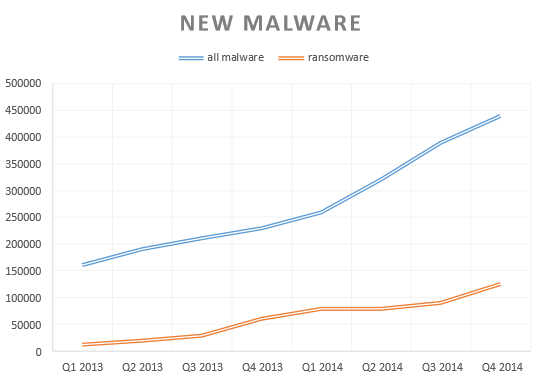
\includegraphics[width=0.45\textwidth]{increase}
\end{figure}

They found most prominently:
\begin{itemize}
\item There are two main Ransomware families (specific pieces of software which have developed over the years). Both with highlighted traits, these are:
\begin{enumerate}
\item TorrentLocker - A Ransomware exclusively distributed by email, and uses the infected user's email address list to distribute further.
\item CryptoWall - Communicates back to the attackers using the Tor network, to remain anonymous.
\end{enumerate}
\item There are a further 97 variants, most of which are related. Some are direct copies however.
\item 35.6\% of the attacks were made by Ransomware that do not perform encryption, but simply delete users files if they do not pay the ransom.
\item CyrptoWall infected 250,000 computers worldwide in the year of publishing (2015).
\end{itemize}Both of the described Ransomware families above are particularly sophisticated according to the author's findings, stating that they both use AES (Advanced Encryption Standard) to encrypt user data. This happens once a user is infected, and because of the high level of security AES was designed for (this method is used by the U.S. government to encrypt classified information for instance \cite{aes}), it makes any attempt at decrypting user data without paying extremely difficult. \par
Although other Ransomware use less sophisticated locking mechanisms such as standard Windows functions as described in the paper, a common user would still not be able to unencrypt the data without the help of good decryption software or with guidance from professionals. The paper noted that it in fact most Ransomware were not concentrating on the strength of the encryption, as long as it took away the ability for users to access files, then they could begin holding such users at ransom. In a whitepaper published by Boromium Security \cite{bromium}, file type targeting is something that can increase the efficiency and speed at which more vital files are encrypted. By only encrypting recently modified, new and common file-type files (as shown in Figure 2.), a Ransomware can cut its footprint and avoid anti-virus systems detecting major file system changes.
\begin{figure}[H]
  \caption{The number of file types encrypted by numerous Ransomware.}
  \centering
  \label{fig:files}
    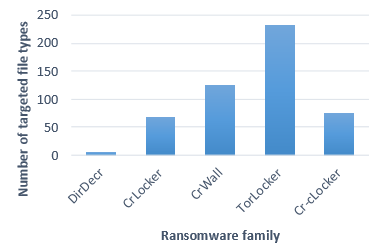
\includegraphics[width=0.45\textwidth]{files}
\end{figure}
The final aspect, and most important part to the process of an attackers infecting a user with the malware is the payment or ransom. In order to remain anonymous, and so that attackers cannot be traced, Bromium noted that nearly all Ransomware used BitCoins as payment. This secure and anonymous payment system allows anyone to send virtual cash through unique BitCoin addresses which can later be traded for cash. \par
Figure 3 shows the most common found way that Ransomware attacks happen. Though with nearly 40\% attacks now affecting multiple platforms, there is a constant shift in means of attacking.
\begin{figure}[H]
  \caption{An example flow of a Ransomware attack.}
  \centering
  \label{fig:order}
    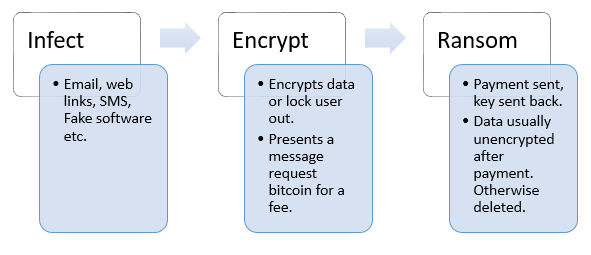
\includegraphics[width=0.45\textwidth]{order}
\end{figure}
\subsection{Transmission of malware}
Although the paper mentioned earlier (A look under the hood) goes into great detail of how Ransomware functions, and the statistics around them, the means at which users receive the malware is very brief in Kharraz's paper. In order to understand how Ransomware is transported, and how this relates to user responsibilities, other papers gave good insight. The Bromium whitepaper listed findings for most common Ransomware attacks:
\begin{itemize}
\item Spam or social engineering
\item Direct or indirect user download
\item Malware installation tools and botnets
\end{itemize}
Where these means of infection relate to the topic of this paper is in the fact that all three contain some user involvement. Without the user clicking on a suspicious link, downloading faulty software, or installing software with unwanted additional add-ons, it could be claimed that malware would not exists or exist in a different manner, as told by K. Wyk \cite{artical}. Because Ransomware realises heavily on user interaction, this is where this form of malware is required to look more professional than traditional viruses or spamming software. \par
The Bromium report highlights the professionalism that is shown from some of the Ransomware seen, and the increase is overall sophistication, making it more believable to be safe software of any kind. As mentioned in the abstract, emails produced to bring users to download the malware has been found to be increasing in sophistication too, with the use of correct user postcodes sent out. Because of this professionalism in the malware produced, software can almost seem to be on the side of the user when trapping them into a ransom. \par

\subsection{The psychology of a Ransomware victim}
A quote made by James Scott from the Institute for Critical Infrastructure Technology said that "Ransomware is more about manipulating vulnerabilities in human psychology than the     adversary's technological sophistication". Although the user may be at ransom with their data, the way in which attackers attempt to convince users to pay is by gaining the trust of a user. To do this various insightful ways have been produced over recent years, such as CryptoWall's method of giving a user one free decryption key in order to make it believable that the attackers actually have the ability to unlock the user's files \cite{paper4}. \par
Images of various Ransomware shown in the Bromium report actually show clear and helpful instructions on how to make payment, and how to decrypt files, again instilling trust with the user. By providing trust, a user will me more inclined to pay, which sets this type of malware apart from any others. Having a user wanting to pay the attackers rather than the attackers having to attempt to steal financial data using more aggressive software makes the work of an attacker in this situation much easier, and more profitable if the attacker can reach the Ransomware to many users. \par

\section{Human errors}
Because humans build and use machines, a mistake by a machine can usually be related back to an error by the human who built it. Therefore, the weakest part of any system appears to be the users, as stated by A Sharaki (Human errors in computer related abuses) \cite{paper1}. The paper points out a number of ways a person can affect the usage and vulnerability of the system, which are not limited to:
\begin{itemize}
\item Fooled, distracted or persuaded
\item Blackmailed- heavily related to Ransomware
\item Be affected by human characteristics such as being tired, idle or apathetic
\end{itemize}
Any of the above can benefit viruses of any kind, making it easier for them to infiltrate computer and networks. Human errors are said to be distinguishable into two types, slips and lapses. Slips could be something such as attaching a wrong file in an email, whilst a lapse would be leaving systems open or unlocked. These two definitions were coined by James Reson (1990) \cite{james}, who compared mistakes to errors, stating that the mistake in the two cases mentioned previously was in not having an adequate plan for checking emails are from reliable sources. A mistake is therefore something that can heavily impact the possibilities of human error. By eradicating mistakes and being more prepared for human error, computer related abuses would be less frequent. \par
In addition to this, the paper by Sharaki noted that human error is part of a human behaviour and that because of many preceding events (or mistakes as mentioned), it may not be the fault of the human. \par
Designers and developers should be aware of the human errors issue, and therefore build mechanisms for dealing with possible errors according to Sharaki. Even if a developer was to create a perfect system with no bugs, or a system that did exactly what it was supposed to do, they should always be designed with any possible misuse in mind. For instance, without blocking every email that comes into a user's system, there will always be a finite number of suspicious emails that will come through the spam filter, and at that point the security lies with the user. In the case of Ransomware, because of the growing advancement of email authenticity this is one example of a hard to avoid mistake without further user training. \par
In addition to the developers, Sharaki also asks for ISPs (Internet Service Providers to protect against spyware and viruses by actively stopping suspicious network activity, which take yet more room for error out of the hands of users.) \par
As stated already, even with many precautions in place, unintentional threat still remains an increasing problem for many organisations or stand-alone users. Alphonso Price (Human factors in information security, 2015) \cite{human-factors} gathered some statistics on mistakes made by users resulting in issues for their respective organisations, and found that 57\% of employees believed that breaches in security caused by accidental or careless users are more damaging as breaches caused by intentionally malicious users. The author believed the reasoning for this lied with the fact that it is easier to predict the subject of attack when done purposely, but unintentional mistakes from other users are unpredictable and harder to forsee. \par
\subsection{Human errors- the consequences}

\section{Conclusion}
The conclusion goes here.

\appendices

\section{}
Appendix two text goes here.
\section*{Acknowledgment}


The author would like to thank...

\ifCLASSOPTIONcaptionsoff
  \newpage
\fi

\begin{thebibliography}{1}

\bibitem{bbc-Ransomware}
BBC Technology News, \emph{The Ransomware that knows where you live}, \hskip 1em plus
  0.5em minus 0.4em\relax \url{http://www.bbc.co.uk/news/technology-35996408} BBC. 2016.
  
\bibitem{paper4}
A.~Kharraz et.al, \emph{Cutting the Gordian Knot: A Look Under the Hood of Ransomware Attacks
},\hskip 1em plus
  0.5em minus 0.4em\relax Northeastern University, Boston, USA. 2015.
  
\bibitem{aes}
Tech Target, \emph{Advanced Encryption Standard (AES)}, \hskip 1em plus
  0.5em minus 0.4em\relax \url{http://searchsecurity.techtarget.com/definition/Advanced-Encryption-Standard}. 2014.
  
\bibitem{bromium}
V.~Kotov and M.~ Rajpal, \emph{Understanding  Crypto-Ransomware},\hskip 1em plus
  0.5em minus 0.4em\relax Bromium Inc, 2015.
  
\bibitem{artical}
K.~van Wyk, \emph{Blaming Users for Virus Chaos?}, 3rd~ed.\hskip 1em plus
  0.5em minus 0.4em\relax \url{http://www.esecurityplanet.com/views/article.php/3377201/Blaming-Users-for-Virus-Chaos.htm}, 2004.
  
\bibitem{paper1}
A.~Sharaki and M.~Nikaram , \emph{Human Errors in Computer Related Abuses},\hskip 1em plus
  0.5em minus 0.4em\relax Journal of Theoretical and Applied Information Technology Vol 47 No 1. 2013.
  
\bibitem{james}
J.~Reason, \emph{Human Error},\hskip 1em plus
  0.5em minus 0.4em\relax Cambridge University Press. 1990.
  
\bibitem{human-factors}
A.~Price and Y.~Choi, \emph{Human Factors in Information Security},\hskip 1em plus
  0.5em minus 0.4em\relax International Journal of Computer and Information Technology, Vol 04 Issue 05. 2015.

\end{thebibliography}

\end{document}


